% !TeX root = ../main.tex

\chapter{工作总结及展望}
\label{cha:Summary}

这篇论文前四章描述了研究工作的理论和实验背景以及相应的物理动机。
%以及一些必要的基础知识等。
论文第~\ref{cha:Xbb}~章展示了一种用于高横动量$H\rightarrow b\bar{b}$事例标定的去质量关联的新算法$D_{Xbb}$,
从研究背景、事例产生、设计思路到算法性能。
它是ATLAS合作组内部推荐的第一个高横动量$X\rightarrow b\bar{b}$事例的标定算法,
在ATLAS合作组内部,
这个新算法的设计方式不仅为以后高横动量$H\rightarrow b\bar{b}$标定算法的开发展现了一种全新的设计方向,
比如即将到来的HL-LHC(High Luminosity Large Hadron Collider)计划~\cite{HLLHC};
也为其他去质量关联的标定算法提供了崭新的思路,比如t夸克和W玻色子标定~\cite{ATL-PHYS-PUB-2017-004}。
而且它可以用于将来与高横动量$H\rightarrow b\bar{b}$过程相关的一系列分析当中,
包括标准模型中希格斯玻色子性质的精确测量~\cite{AHbb6,AHbb7,AHbb8,AHbb5},
可以显著提升高横动量区间$H\rightarrow b\bar{b}$过程的信号灵敏度。
它也可以用于一部分与超出标准模型的新物理~\cite{BSMHIGGS1,BSMHIGGS2,BSMHIGGS3,DXBB6,DXBB7}相关的分析当中,
这些新物理模型能与标准模型中希格斯玻色子耦合,
部分模型中的新粒子质量比较大,能衰变产生高横动量的希格斯玻色子,
更能发挥新算法$D_{Xbb}$的优势,
其中正在使用这个新算法$D_{Xbb}$的物理分析有两个:
其中一个是通过在衰变末态包含一个标准模型中希格斯玻色子的衰变道来寻找暗物质媒介子$Z'$~\cite{DXBB4,DXBB5,DXBB6},
如图~\ref{fig:ENDING1}~所示是过程所对应的费曼图,产生的暗物质媒介子$Z'$会衰变成一个赝标量粒子A和一个标准模型的希格斯玻色子,
其中A随后衰变成两个暗物质费米子$\chi$,而希格斯玻色子随后衰变成$b\bar{b}$夸克对,
在上一轮类似分析的基础上~\cite{DXBB3},
这一轮分析将会用到$Run\_2$计划收集的全部数据和新算法$D_{Xbb}$用于标定高横动量$H\rightarrow b\bar{b}$过程;
另一个是通过在衰变末态包含一个标准模型中希格斯玻色子的衰变道寻找超出标准模型的重规范玻色子Y~\cite{DXBB7,DXBB8,DXBB9,DXBB10,DXBB11},
图~\ref{fig:ENDING2}~为相应的费曼图,重粒子Y可以衰变道一个新玻色子X和一个标准模型的希格斯玻色子,
其中X随后衰变成标准模型的两个夸克,而希格斯玻色子随后衰变成$b\bar{b}$夸克对,
同样基于上一轮类似分析~\cite{DXBB2},现在的这个分析会使用$Run\_2$计划期间的所有数据和新算法$D_{Xbb}$。
基于新算法$D_{Xbb}$优异的性能,有望能显著提高新物理信号的搜索灵敏度。

\begin{figure}
  \begin{center}
    \includegraphics[width=0.5\textwidth]{figuresEND/DMZHA.pdf}
  \end{center}
  \caption{
利用$Z' \to H+A\to b\bar{b}+\chi\bar{\chi}$衰变来寻找暗物质。其中是$Z'$暗物质媒介子,H为标准模型中希格斯玻色子,A为赝标量粒子,$\chi$为暗物质费米子。
  }
    \label{fig:ENDING1}
\end{figure}

\begin{figure}
  \begin{center}
    \includegraphics[width=0.5\textwidth]{figuresEND/YXH.pdf}
  \end{center}
  \caption{
利用$Y\to H+X\to b\bar{b}+q\bar{q}$衰变来寻找超出标准模型的重规范玻色子。其中Y是所寻找的重规范玻色子,H为标准模型中希格斯玻色子,X为一个新粒子。
  }
    \label{fig:ENDING2}
\end{figure}

论文第~\ref{cha:Dijet}~章呈现了物理分析在双喷注末态事例中寻找新物理的动机、事例重建和筛选过程、b-jet标定算法、本底估计策略和搜索技术以及结果,
这是b-jet标定算法DL1r以77\%的工作点第一次用于ATLAS实际的物理分析当中, 
%并对衰变末态包含b-jet的信号的搜索灵敏度有了显著的提升,
利用ATLAS探测器在$Run\_2$计划期间收集的所有数据,我们并没有发现显著的新物理信号,并且对多个基准模型设置了更加严格的排除限。
对于大部分基准模型,这个分析的结果给出了目前为止最严格的限制~\cite{DIJETSUM},比如对于暗物质$Z'$模型,
图~\ref{fig:ENDING3}~展示的是ATLAS合作组不同分析中强子型衰变的轴矢量$Z'$模型中耦合常数$g_q$即$g_{SM}$的$95\%$置信度上限随着信号质量的变化,
深橙色的线表示我们得到的排除限结果,左上方的区域在95\%的置信度下将会被排除,可以看到这个结果比之前的结果更加严格。
随着将来LHC的升级改造~\cite{HLLHC},如图~\ref{fig:HLLHC}~所示,在2027年,高亮度大型强子对撞机(High Luminosity Large Hadron Collider, HL-LHC)将正式开始运转,
并计划将质心系能量提高到14GeV,而且数据总积分亮度将大大增大,达到3000$fb^{-1}$,
这也将大大提升双喷注末态新物理的搜索灵敏度。



\begin{figure}
  \begin{center}
    \includegraphics[width=0.75\textwidth]{figuresEND/ZPRIME.png}
  \end{center}
  \caption{ 
  ATLAS合作组不同分析中强子型衰变的轴矢量$Z'$模型中耦合常数$g_q$即$g_{SM}$的$95\%$置信度上限随着信号质量的变化。
  实线表示观测到的排除限,虚线表示预期的排除限。
   }
    \label{fig:ENDING3}
\end{figure}



\begin{figure}
  \begin{center}
    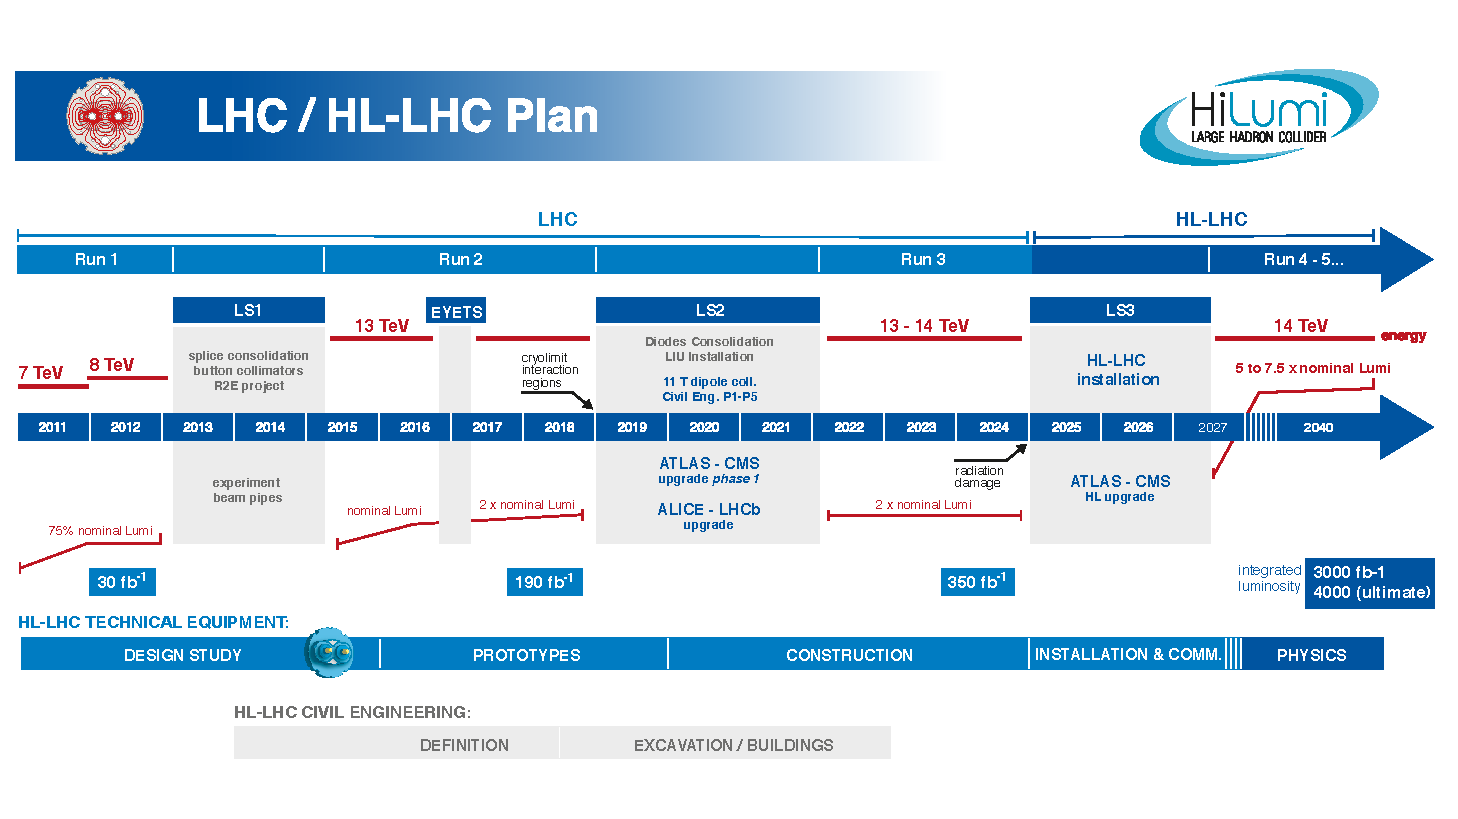
\includegraphics[width=0.75\textwidth]{figuresEND/HLLHC.pdf}
  \end{center}
  \caption{
高亮度大型强子对撞机(HL-LHC)计划。
  }
    \label{fig:HLLHC}
\end{figure}



